\chapter{An Introduction to the Cape of Good Hope Telegraphs }


\section{Cape of Good Hope Telegraph Company 1860}

The first telegraph line in southern Africa was inaugurated on 6th May 1860 
at the Cape of Good Hope.

It operated as a private enterprise, owned by the "Cape of Good Hope 
Telegraph Company". 

The Company operated a line between Cape Town and Simonstown.  Its first office 
was a wooden, pagoda-like structure on the comer of Adderley and Strand Streets. For a very good historical account of telegraphs see the Telegraph Office.
Pagoda
The first Telegraph Office. Operated in a Pagoda like structure at the 
Corner of Adderley and StrandsStreets in Cape Town at the Cape of Good Hope

\begin{marginfigure}
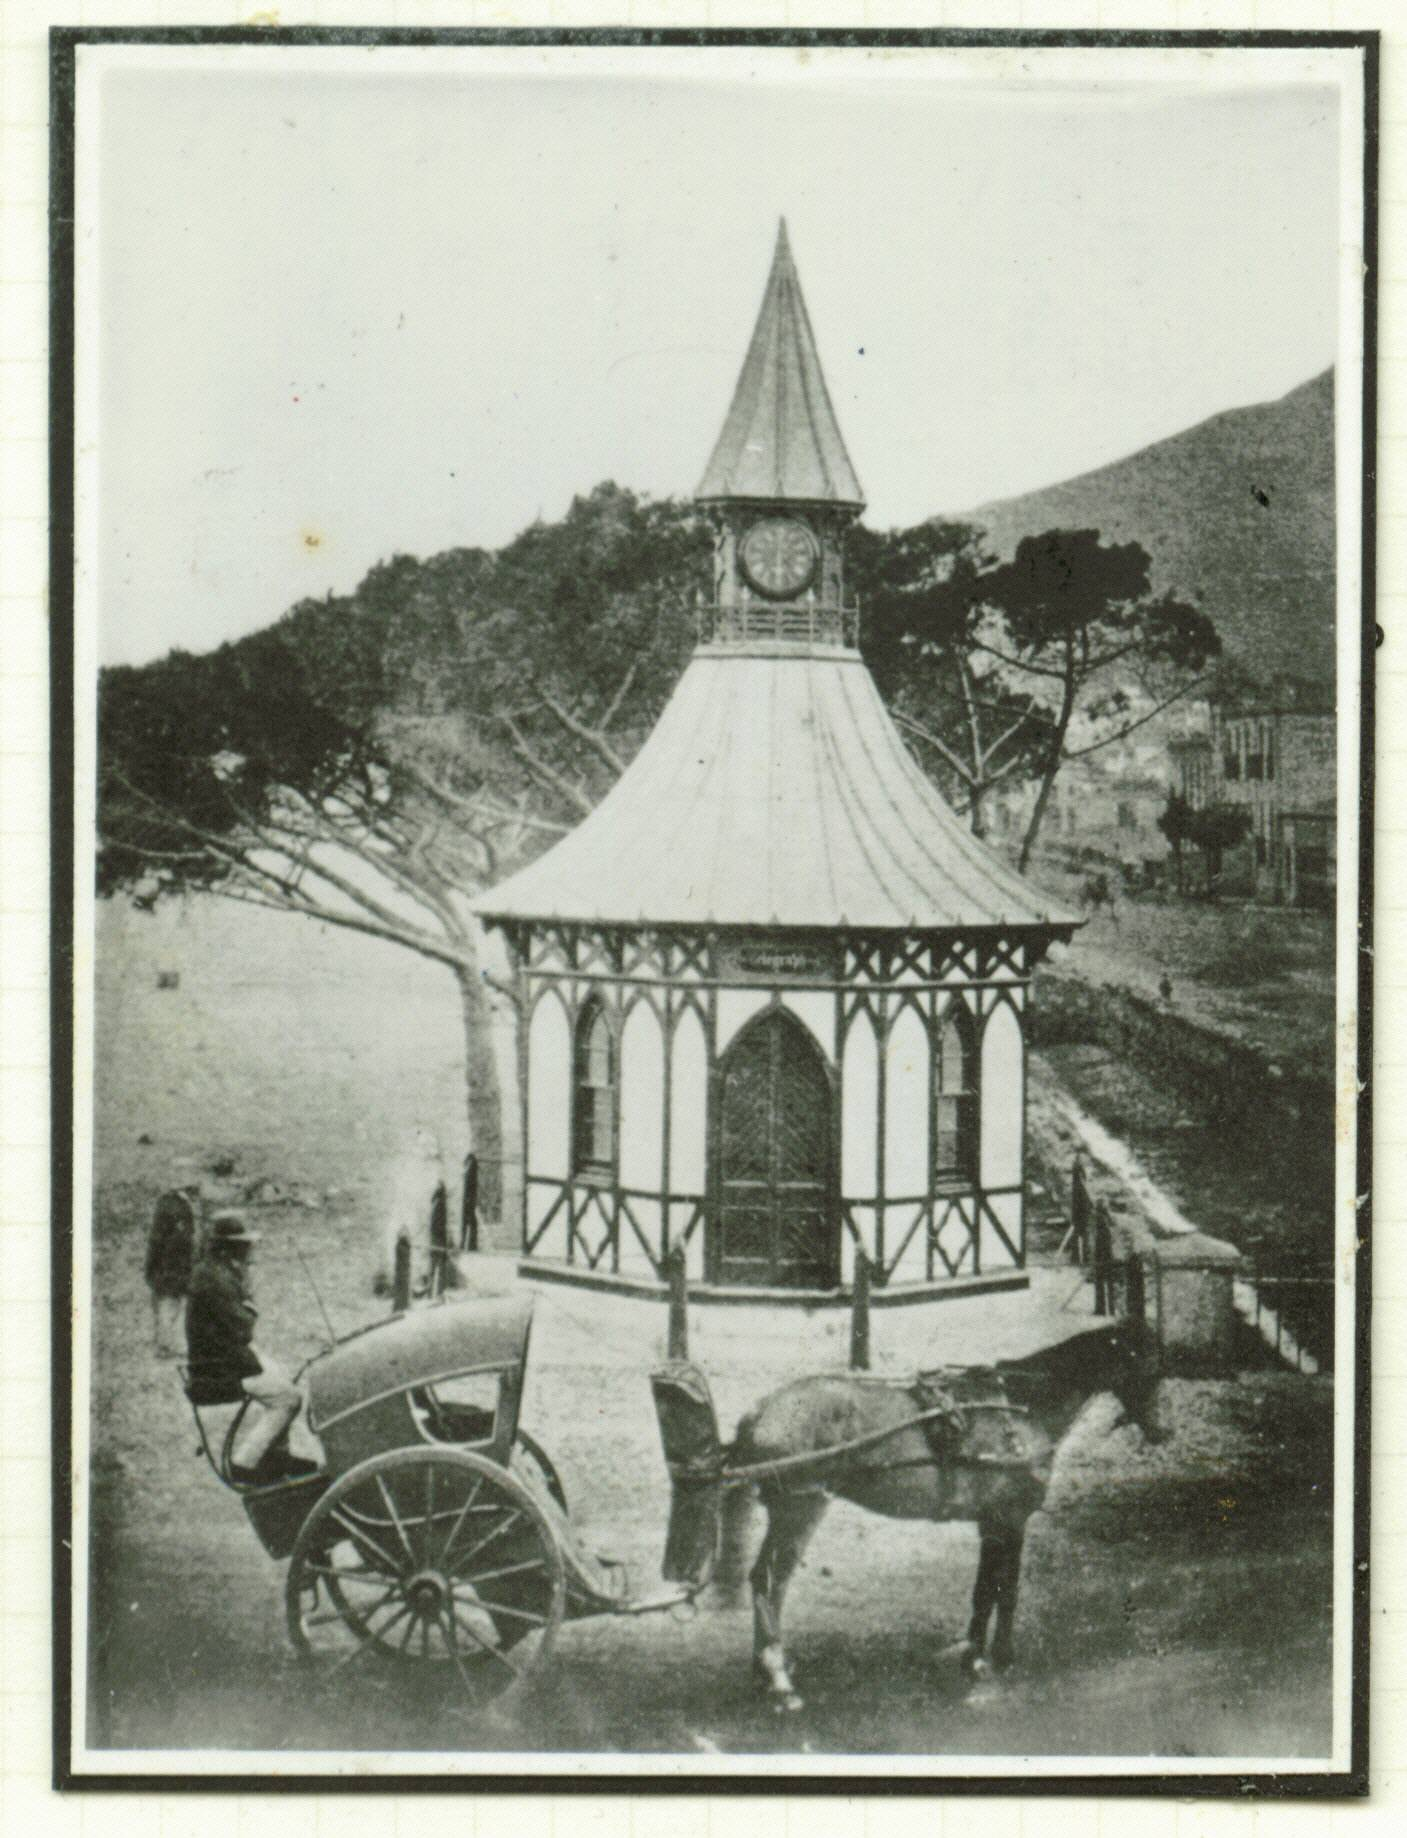
\includegraphics[width=0.95\textwidth]{../cape-of-good-hope/telegraph-office/Pagoda.jpg}
\caption{
 The first Telegraph Office. Operated in a Pagoda like structure at 
 the Corner of Adderley and StrandsStreets in Cape Town at the Cape 
 of Good Hope.
}
\end{marginfigure}

\section{Cape of Good Hope Telegraphs 1873}

 
 
A line from East London to King Williamstown was installed in 1861 and 
further extensions linked Port Elizabeth and Grahamstown. The government 
subsidized this line. In 1863 telegrams could be accepted for East London, 
King Williamstown, Port Elizabeth and Grahamstown. Other extensions followed. 
With the discovery of diamonds, the wooden pagoda of the telegraph office became 
a vital centre of commercial and financial activity for Cape Town's 
business community.

\section{1873 Government Control}

On the 1st July, 1873, the lines of the Company became the property of the 
Government by purchase for the sum of \pound41,123, under Act No, 18 of 1872, 
and  from that date were worked by the Telegraph Department. 
(Until 16 February 1885, however, 
it remained a separate entity). At the time of the transfer the entire 
length of telegraph 
line in the Colony was 760 miles, with 16 Offices.
1883

The first South African Telegraph Union Convention was entered into between 
the Cape Colony, Natal and the 
Orange Free State in 1883. This agreement effected the abolition of the 
system of double inland rates for telegrams exchanged between the countries, 
parties to the Convention, and brought the tariff for such messages down to 
the level of the rates in force within the Cape Colony
(The expansion of the Telegraph Services are largely attributed 
to the efforts of the then Postmaster-General the Cape of Good Hope Sir S R French).

\section{1892 Telegraph Service Extended to Basutoland}

In 1892 a Telegraph Service was inaugurated in the Crown Colony of 
Basutoland under the administration of the Postmaster-General of the 
Cape Colony; and in the following year the telegraphs of the British 
South Africa Company were also placed under the management of the 
Postmaster-General of this Colony, and remained so until the 23rd February, 1897.
1895 Incorporation of British Bechuanaland Telegraphs into Cape of Good Hope


By the annexation of British Bechuanaland to the Cape Colony in November, 1895, 
the telegraph system in that territory became a part of the 
general system of the Cape Colony.

\chapter{1899
} 
In 1899 the telegraph rates within the Cape Colony and to the Transvaal, 
Natal and the Orange Free State were
again revised, the rate being fixed at 1d. per word with a minimum charge of 1s.
1901







A third telegraphic connection between South Africa and Europe, in the form of a 
direct deep-sea cable from Porthourno, Cornwall, to Table Bay, via St. Vincent, 
Ascension and St. Helena, was opened in 1901; and the following year direct 
communication 
between South Africa and Australia was 
established by means of a cable landed at Durban, with which the 
Western Cable was 
connected by a special overland line from Cape Town, constructed 
exclusively for the cable traffic.


As a result mainly of negotiations initiated and carried through by this 
Department, considerable reductions
have been effected in the rate charged by the Eastern and South African 
Telegraph Company for cablegrams between South Africa and Europe. 
From the following table it will be observed that during the last 
ten years the rate has been reduced 50 per cent., and that, allowing 
for the extraordinary inflation of the figures covering the period of 
the war, the number of cablegrams forwarded from Government Telegraphic 
Offices in the Colony indicate substantial increase in the traffic since 1899. -
Post Office Telegraphs of the Cape of Good Hope 1885


\ph[width = .60\textwidth]{../cape-of-good-hope/telegraph-office/telegram.png}{
Cape telegram handed in at Beaufort west and received 
Graaf-reinet (July 1902). Reply was prepaid.
}

Post Office telegraphs were incorporated under the aegis of the 
postmaster general in 1885. A typical handstamp in use in the 1870s (TO 1) 
was oval and contained the words "Telegraph Office" and the place name in 
the upper and lower curves, respectively. The earliest types of dated strikes 
of the Telegraph Office under government control---but not yet under 
postal administration---are TO 2 to 6, and those from 1885 onwards, 
when the office fell under the General Post Office, are TO 7 to 10. (TO 11 and 12).
Telegraph Office
 

The country post offices of the Cape of Good Hope also used the telegraph 
datestamps somewhat indiscriminately for defacing stamps on mail. As a result, 
they were withdrawn and the normal datestamp used for dating telegrams. 
Some postmasters used the Barred Oval Numeral Canceller (BONC) for this purpose.

The head office in the General Post Office in Cape Town, however, continued using a special stamp for dating telegrams and adhesives canceled at this office can accordingly be easily identified. Although all the old telegraph forms were destroyed from time to time under the supervision of postal officials in terms of standing instructions, in several instances the stamps were first removed and thus escaped destruction. From about 1905 onwards, the Cape Town head office also used the ordinary datestamps to cancel the stamps on telegrams.

As regulations prohibiting the removal of stamps from telegraph forms were now more rigorously enforced, 
fewer stamps with telegraphic cancellations are extant. 
They are seldom seen and are usually on the 6d., Is. and 5s. values of 
the King Edward VII issue of the Cape of Good Hope. 

Telegraph offices were also established at railway station post 
offices and these (RTO 1 and 2) can be identified by the use of 
the letters R.T.O. for Railway Telegraph Office at the bottom of the postmark.  
    
\ph[width = .90\textwidth]{../cape-of-good-hope/RTO1.jpg}{Letter posted in the Telegraph and Railway Office in
Ludlow, bears RTO1 postmark in violet and receiving Cape Town CDS t the back. }



          